% COMPLEX NETWORKS 2026 — extended abstract track (Springer LLNCS format,
% template CNALatexTemplate_Abstract; recommended 2-3 pages, hard max 4).
% Build: tectonic main.tex   (figures referenced from ../figures, regenerated
% by `python figures/make_all.py`; all statistics derive from
% paper/numbers.json via paper/extract_numbers.py — no hand-typed numbers).
\documentclass{llncs}
\usepackage{mathptmx}
\usepackage{helvet}
\usepackage{courier}
\usepackage{graphicx}
\usepackage{amsmath,amsfonts}
\usepackage[bottom]{footmisc}
\renewcommand{\topfraction}{.95}
\renewcommand{\textfraction}{.05}
\renewcommand{\floatpagefraction}{.9}
\setcounter{topnumber}{2}
\setlength{\textfloatsep}{6pt plus 2pt minus 3pt}
\setlength{\abovecaptionskip}{4pt}

\begin{document}

\title{Seeding complex contagions in modular organizations:\\
a reach--retention trade-off}
\titlerunning{Seeding complex contagions in modular organizations}
\author{Paul Bufort}
\authorrunning{P. Bufort}
\institute{Independent Researcher --- ORCID 0009-0000-6080-1887\\
\email{paulbufort@paulbufort.com}}

\maketitle

\begin{abstract}
Folklore holds that costly behaviors are best spread by seeding dense
clusters; the wide-bridges literature supplies the rationale. We revisit this
on synthetic two-layer organizations---a formal hierarchy plus an informal
network of dense small teams---with fractional-threshold dynamics
(heterogeneous thresholds, innovator atom, credibility-weighted exposure,
ready\slash willing\slash able gating). Under equal seed budgets (broadcast
excepted): (i)~broadcast converts only innovators---zero adoption without
them in every run; (ii)~contrary to folklore, \emph{scattered} seeding beats
cluster seeding on reach in this modular regime, where every seed is already
embedded in a dense team; (iii)~under reinforcement-dependent decay the
advantage \emph{collapses to parity}: a reach--retention trade-off, not a
dominant strategy; (iv)~global visibility acts exactly as threshold
inflation ($\theta/v$); seed-targeted visibility pays in proportion to
outward credibility. All
data are synthetic; results are bit-for-bit reproducible from one master
seed.
\keywords{complex contagion, threshold models, seeding strategies,
organizational networks, agent-based simulation}
\end{abstract}

\section{Introduction and related work}

Threshold models~\cite{granovetter1978} formalize why costly behaviors spread
differently from information: adoption requires reinforcement from multiple
credible sources. Cascades on random graphs obey a vulnerability
boundary~\cite{watts2002}; \emph{complex contagions} need wide bridges of
overlapping ties, which long-range shortcuts destroy~\cite{centola2007,centola2010}.
Network-intervention practice~\cite{valente2012} distilled this into a popular
prescription: \emph{seed dense clusters, never scatter}---evidenced largely in
populations not otherwise embedded in cohesive groups. Adjacent results
strain it: modularity aids cascades only up to an
optimum~\cite{nematzadeh2014}; dispersed neighbor seeding beats clustered
seeding in threshold models~\cite{ou2022}; seed placement is its own
measurement problem~\cite{guilbeault2021,tanase2026}; and random ties match
or beat clustered ties on reach unless interest decays
fast~\cite{wan2025,sassine2024}---a structural reach--reinforcement
trade-off whose seeding-strategy analogue we test at fixed topology. Real
organizations are \emph{modular}---nearly everyone already sits inside a
dense small team---so what does cluster seeding buy when every seed is
already surrounded by a cluster? We study this with a transparent
mechanistic agent-based model, with every modeling decision logged
alongside the code (Sect.~\ref{sec:discussion}).

\section{Model}
\label{sec:model}

A generator produces two-layer organizations: a formal hierarchy (CEO, 8
departments, $\sim$250 teams of mean size 8) and an informal influence
network---dense within teams ($p{=}0.9$), locally concentrated between
ring-adjacent ``sister'' teams, sparse across departments (silo
$s{=}0.85$), plus tenure-homophilous noise; adoption propagates on the
informal layer only. Agent $i$ holds threshold
$\theta_i \sim \mathrm{Beta}(\mu\kappa,(1-\mu)\kappa)$, $\mu{=}0.30$, and with
probability $p_{\mathrm{innov}}{=}0.025$ is an \emph{innovator}
($\theta_i{=}0$). Exposure is the credibility-weighted share of contacts whose
adoption is visible,
\begin{equation}
\mathrm{share}_i(t) = \frac{\sum_{j\in N(i)} v_j\, w_{ij}\, a_j(t{-}1) + b(t)}
                           {\sum_{j\in N(i)} w_{ij} + b(t)},
\label{eq:share}
\end{equation}
with credibility $w$ (close collaborator $1.0>$ manager $0.7>$ distant peer
$0.6>$ central comms $0.3$), source visibility $v_j\in[0,1]$ (default 1), and
$b(t)$ a transient comms term active only while a broadcast runs. Adoption
requires \emph{ready} ($\mathrm{share}_i\ge\theta_i$ and $\mathrm{share}_i>0$,
i.e.\ awareness), \emph{willing} (Bernoulli $0.85$), and \emph{able} ($1.0$
here); updates are synchronous. Optional decay: adopters relapse with
probability $\rho$ per step while $\mathrm{share}_i<\theta_i$. Four
seeded strategies share a $5\%$ budget ($100$ of $N{=}2000$): \emph{random},
\emph{champions} (top informal degree), \emph{cluster} (whole teams),
\emph{line-managers-first}; \emph{broadcast} is a zero-seed awareness
baseline (one universal low-credibility pulse, not a seed budget)---fixed
structural heuristics, not influence-maximization
optima~\cite{kempe2003,ou2022}. Each condition: 50 replicates (sweeps: 12), fresh
organization each, one master seed.\looseness=-1

\section{Results}
\label{sec:results}

\textbf{Reach (Fig.~\ref{fig:headline}).} At $\kappa{=}20$, broadcast converts
essentially only the innovators, stalling at $5.5\pm3.4\%$ (mean$\pm$SD; range
1.8--14.5\%); cluster seeding builds local critical mass and reaches
$31.9\pm9.2\%$ before silos cap it---the distributions do not overlap across
$2\times50$ replicates (broadcast max $14.5\%<$ cluster min $17.1\%$). But the
cluster-seeding prescription fails here: \emph{scattered} strategies dominate
reach (random $69.5\pm11.1\%$, champions $73.4\pm7.0\%$). The mechanism is
mesoscopic: random spreads its 100 seeds over $84\pm3$ teams (champions
$60\pm5$) vs cluster's $13\pm1$ saturated ones, igniting $\sim$200 of 249
teams to majority (random $197\pm34$, champions $207\pm22$) vs cluster's
$89\pm27$---mostly by inter-team spillover (random: $125$ of $197$
unseeded).\looseness=-1 Under broader heterogeneity ($\kappa{=}12$) broadcast becomes a lottery
($19.8\pm12.5\%$, range 4.9--64.5\%); the ordering is unchanged. Which regime
a real organization inhabits is open: thresholds are unobserved.

\begin{figure}[t]
\centering
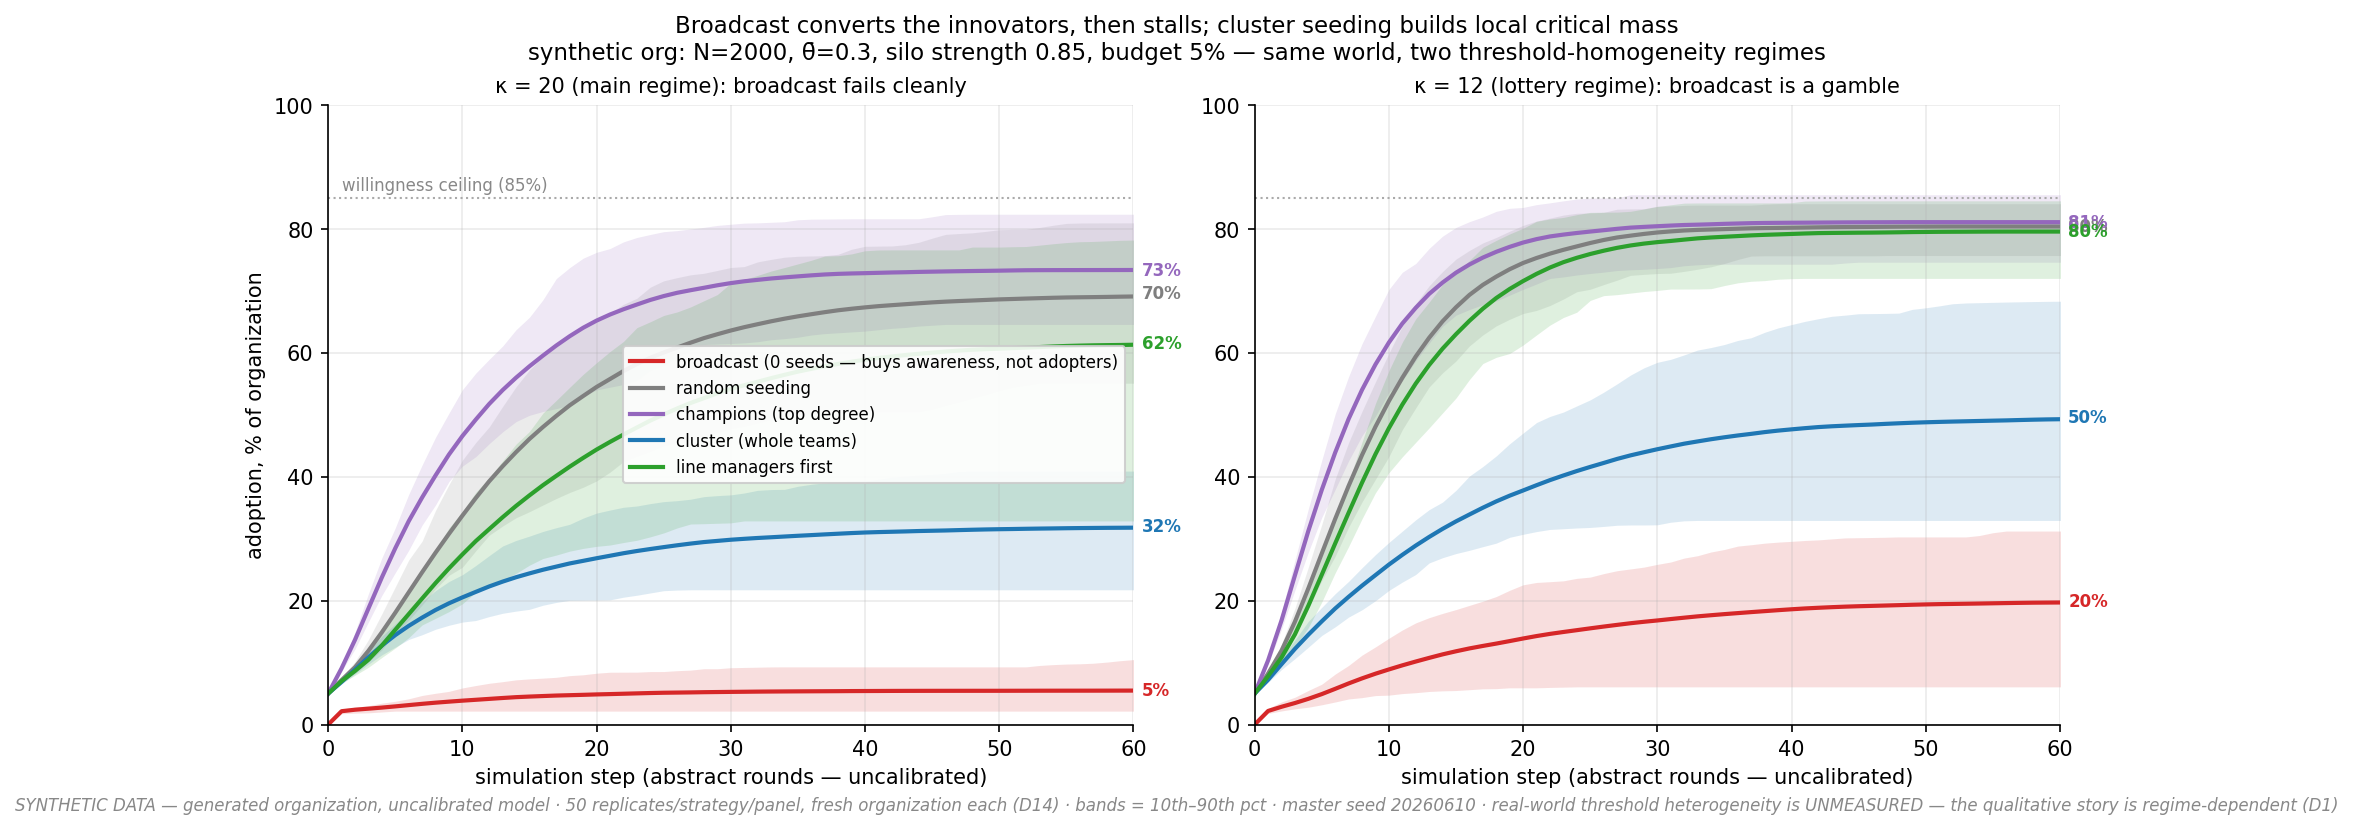
\includegraphics[width=.70\textwidth,trim={0 0 0 0.55in},clip]{../figures/headline.png}
\caption{\textbf{Synthetic data.} Four equal-seed-budget strategies plus the
zero-seed broadcast baseline in two regimes ($N{=}2000$, $\bar\theta{=}0.30$,
silo $0.85$, budget $5\%$; 50 replicates/strategy/panel; bands: 10th--90th
pct). Broadcast fails cleanly at $\kappa{=}20$, gambles at $\kappa{=}12$;
scattered beats cluster in both.}
\label{fig:headline}
\end{figure}

\textbf{Innovators carry broadcast---not the scattering advantage
(Fig.~\ref{fig:pinnov}).} At $p_{\mathrm{innov}}{=}0$, broadcast converts
$0.0\%$ in all 12 replicates---observed, not a theorem: its yield is
entirely innovators.
Yet random still beats cluster ($41.4\pm9.3\%$ vs $20.1\pm4.3\%$): team
embedding plus the threshold tail suffices. Sustained campaigning does not repair the arithmetic: 20 steps
lift broadcast only to $11.6\%$---a third of cluster, a sixth of
scattering.\looseness=-1


\begin{figure}[t]
\begin{minipage}[t]{.36\textwidth}
\centering
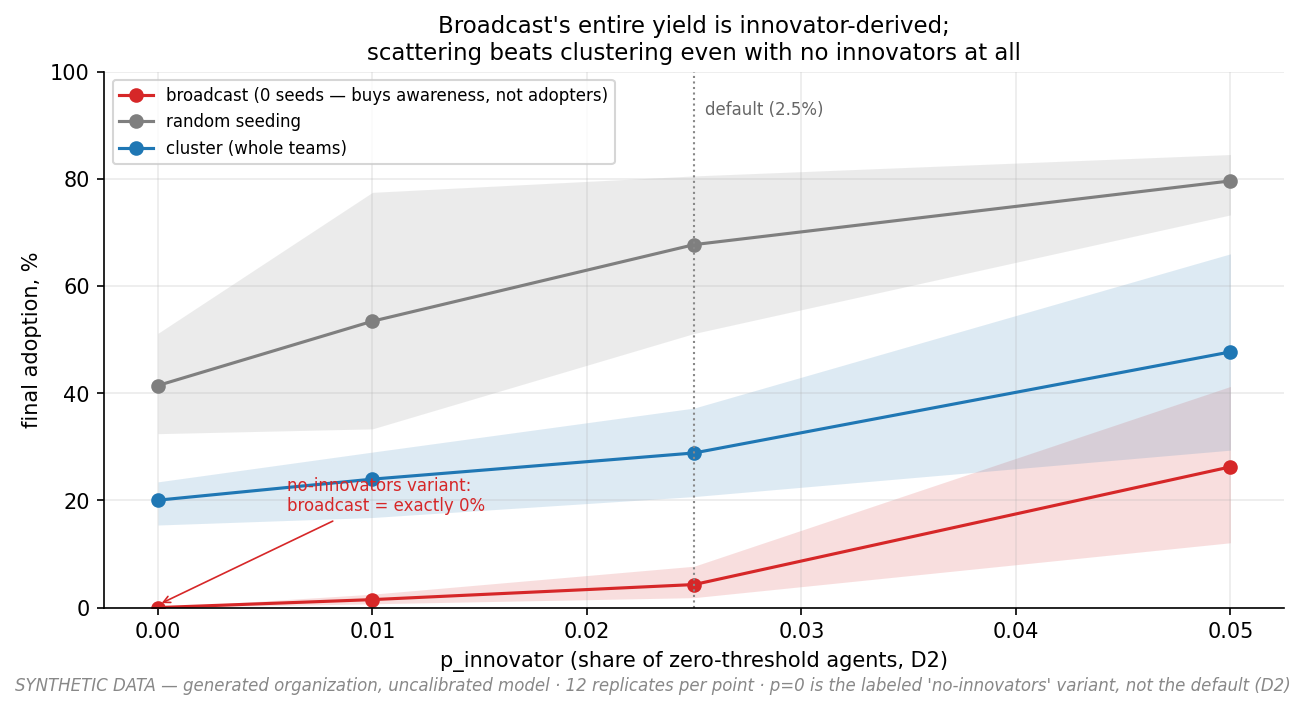
\includegraphics[width=\textwidth,trim={0 0 0 0.42in},clip]{../figures/exp1_pinnov.png}
\caption{\textbf{Synthetic data.} Final adoption vs innovator share (12
replicates/point; otherwise as Fig.~\ref{fig:headline}, $\kappa{=}20$). At
$p{=}0$ broadcast converts zero in all runs; scattered $>$ cluster
survives.}
\label{fig:pinnov}
\end{minipage}\hfill
\begin{minipage}[t]{.50\textwidth}
\centering
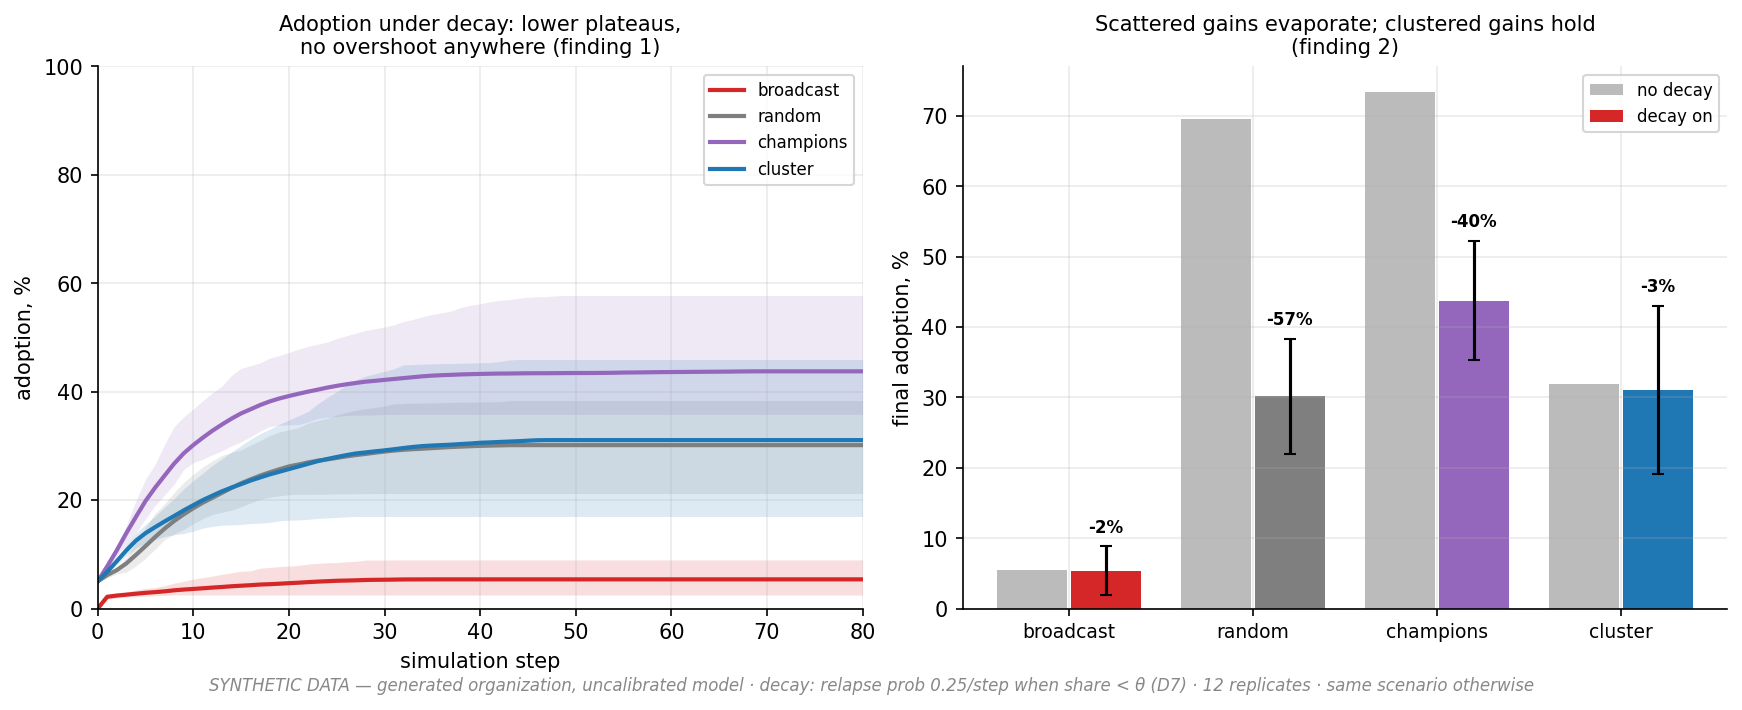
\includegraphics[width=\textwidth]{../figures/exp1_decay.png}
\caption{\textbf{Synthetic data.} Reinforcement-dependent decay
($\rho{=}0.25$; 12 replicates; otherwise as Fig.~\ref{fig:headline},
$\kappa{=}20$). Left: curves; right: decay off/on. Scattered reach is
fragile; clustered adoption locked in.}
\label{fig:decay}
\end{minipage}
\end{figure}

\textbf{Decay erases the reach advantage (Fig.~\ref{fig:decay}).} With
reinforcement-dependent relapse ($\rho{=}0.25$ while
$\mathrm{share}<\theta$), scattered gains largely evaporate---random
$69.5\%\rightarrow30.1\%$ ($-57\%$), champions $-40\%$---while cluster-seeded
adoption is nearly unaffected ($31.9\%\rightarrow31.1\%$, $-2.7\%$, n.s.): every
adopter in a saturated team stays surrounded by adopters. The gap is no
longer detectable ($+0.9$\,pp, 95\% CI $[-8,+10]$, $n{=}12$); scattered
collapses \emph{toward} cluster, not below it---a clean reversal needs higher
relapse. No strategy dominates both objectives: a \emph{reach--retention
trade-off}. (Decay never produces the documented ``spike-then-relapse''
shape---relapse interleaves with adoption; a negative result we report, not
hide.)\looseness=-1


\textbf{Visibility: a theorem and an intervention (Fig.~\ref{fig:pilots}).}
From Eq.~\eqref{eq:share}, the trajectory under global visibility
$(\{\theta_i\},v)$ is \emph{identical} to $(\{\theta_i/v\},1)$ in any
broadcast-free scenario, decay included (exact;
machine-verified). Invisibility is threshold inflation: it starves every strategy
toward the broadcast floor ($v\le0.6$: no strategy exceeds $8.8\%$). A
global $v$ acts only through rescaled thresholds---in principle these can
reorder strategies; in the tested range scattered vs cluster never
flips---broadcast alone is exempt (loud by nature). Only
\emph{differential} visibility matters: seeds at full visibility
(``observable pilots'') at
$v_{\mathrm{global}}{=}0.8$ yield $+4.0$\,pp (cluster), $+9.5$\,pp (random),
$+15.0$\,pp (champions)---proportional to outward credibility per seed
($5.7/11.7/16.1$): a pilot team's megaphone mostly points at people who
already adopted. It does \emph{not} rescue cluster seeding.\looseness=-1

\begin{figure}[t]
\centering
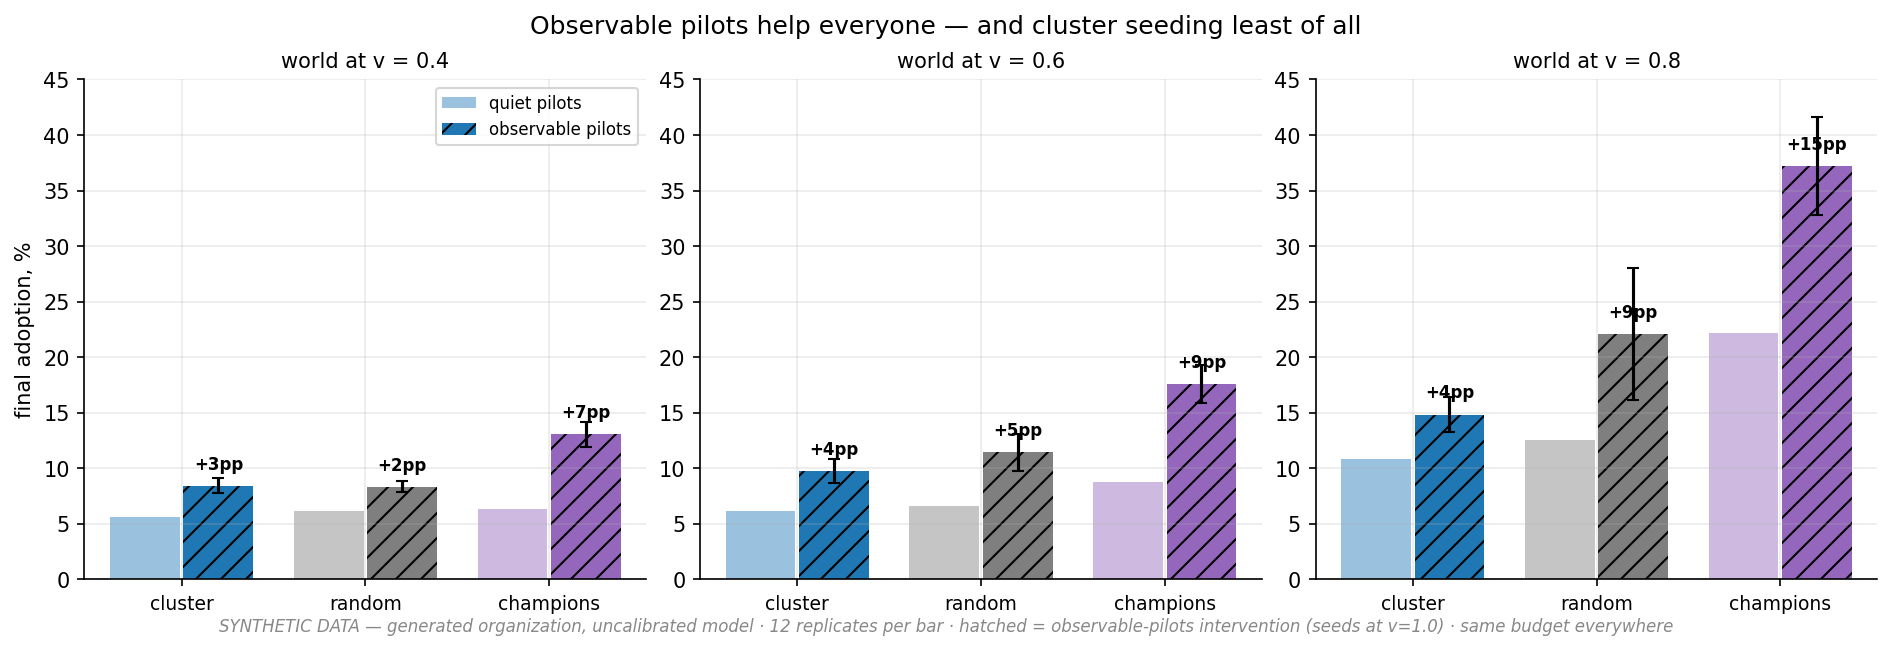
\includegraphics[width=.48\textwidth,trim={0 0 0 0.32in},clip]{../figures/exp3_pilots.png}
\caption{\textbf{Synthetic data.} Observable pilots: seeds at $v{=}1$, world
at $v_{\mathrm{global}}$ (12 replicates; hatched: on). Gains track outward
credibility; cluster benefits least.}
\label{fig:pilots}
\end{figure}

\section{Discussion}
\label{sec:discussion}

The meso-structure overturns the micro-level prescription: once everyone
lives in a dense team, guaranteed local reinforcement---cluster
seeding's defining asset---is no longer scarce; scattering buys more
ignition surface per budget. What survives is conditional: under
reinforcement-dependent decay, cluster seeding is the \emph{retention}
strategy, not the reach strategy---the seeding-level counterpart of the
structural reach--reinforcement trade-off~\cite{wan2025,sassine2024}.
All of this holds \emph{within a
synthetic, uncalibrated model family}: thresholds unobserved, time abstract,
one behavior in isolation; a 19-entry limitations file ships with the code.
Next: a dispersed--cluster regime map ($\bar\theta\times$budget).\looseness=-1

\emph{Reproducibility.} Every modeling decision (D1--D17) is logged with
alternatives and arbitration status; limitations and non-reproductions ship
with the code. CI fails if any published number changes; all statistics are
machine-extracted from versioned results. Repository: AGPL-3.0, public at
publication.\looseness=-1

\bibliographystyle{splncs03}
\vspace{-11pt}
\bibliography{refs}

\end{document}
